\section{SeeDB System Architecture}
\label{sec:architecture}

Figure \ref{fig:sys-arch} shows the architecture of our system. Currently,
\SeeDB\ is a wrapper around a database. While optimization opportunities are
restricted by virtue of being outside the DBMS, we believe that this design
allows quick iteration and permits \SeeDB\ to be used with a variety of
databases.

\begin{figure}[htb]
\centerline{
\hbox{\resizebox{9cm}{!}{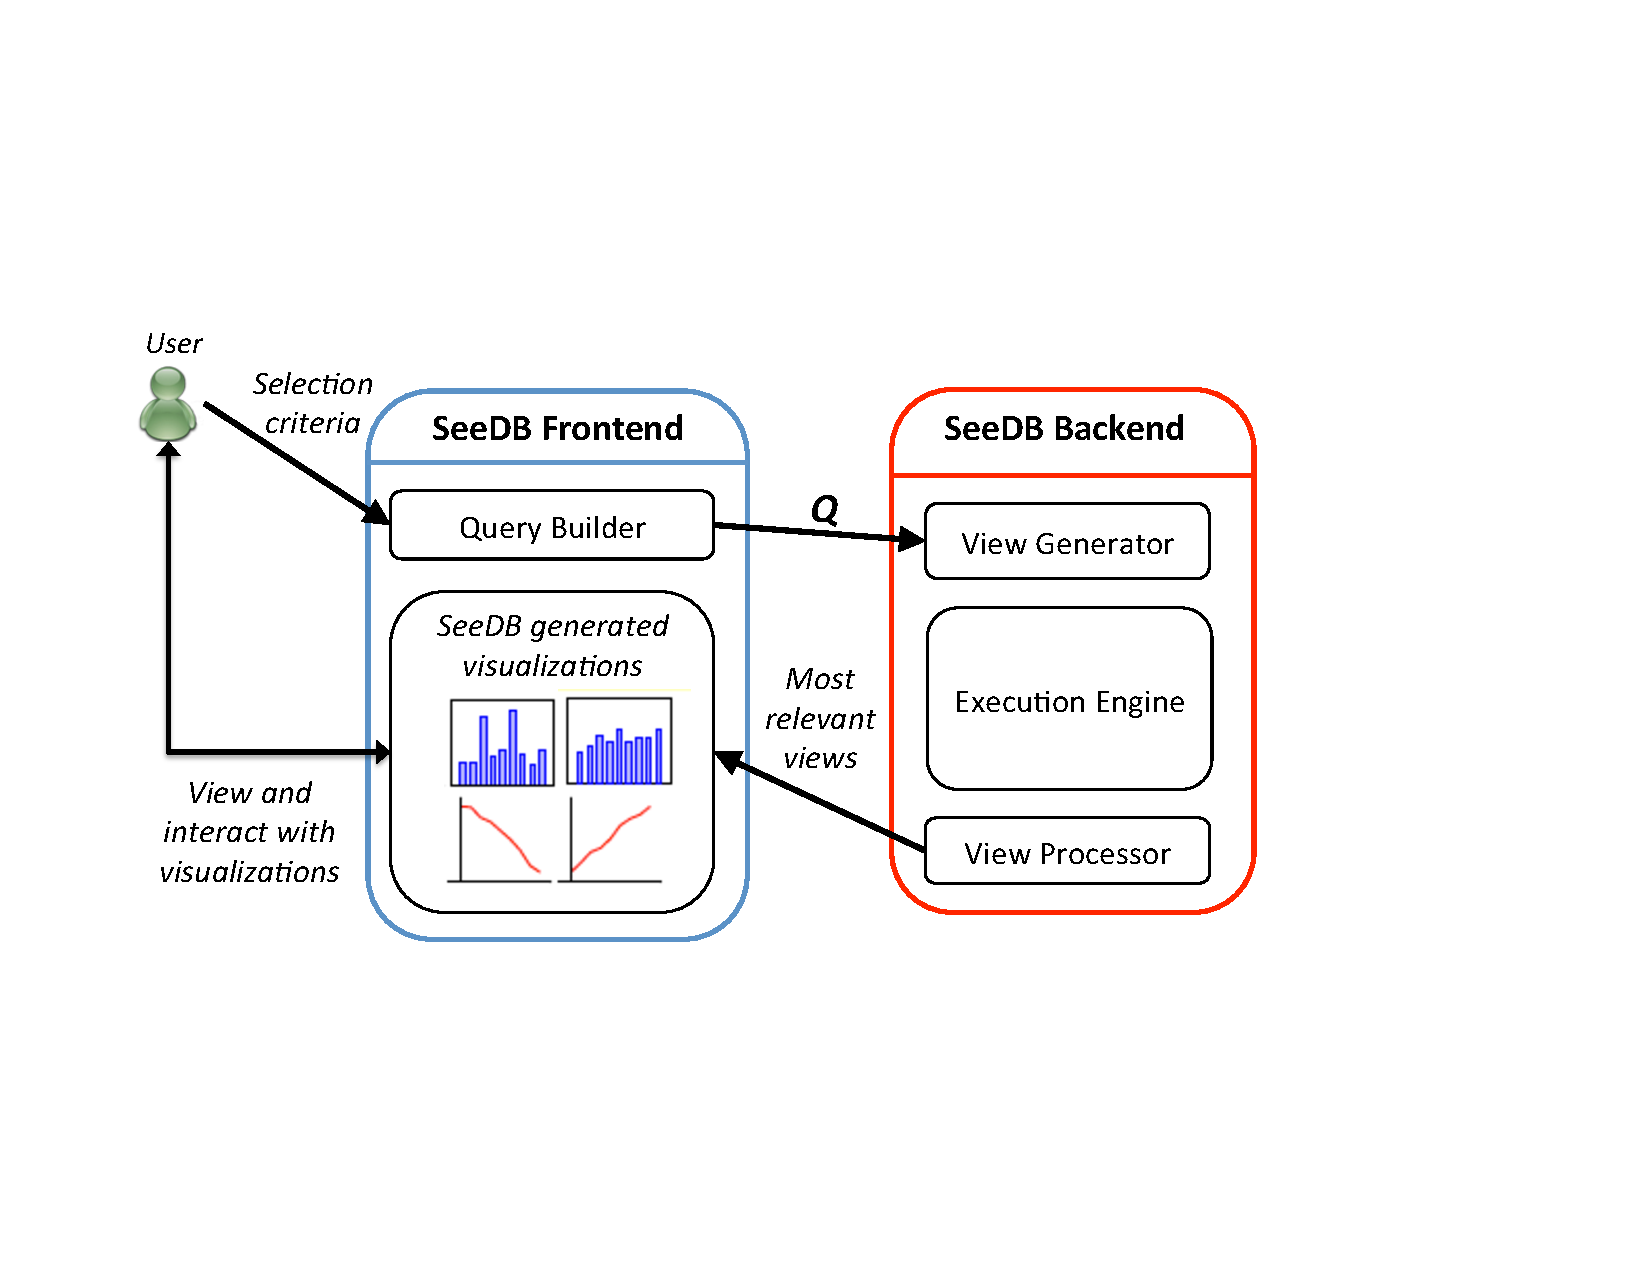
\includegraphics[trim=10mm 50mm 10mm 50mm,
clip=true]{Images/seedb-architecture.pdf}}}}
\caption{SeeDB Architecture}
\label{fig:sys-arch}
\end{figure} 

The \SeeDB\ front end allows the user to make queries to the \SeeDB\ backend
through several means including raw SQL, via a query-builder and via
pre-formulated queries (more in Section \ref{subsec:seedb_frontend}). Once user
queries are sent to the backend, the Metadata Collector queries the relevant
tables for information such as table sizes, column types, table statistics etc.
This metadata is essential for the subsequent processing performed by \SeeDB\.
The user queries along with metadata are then sent to the Query Generator.
The purpose of the Query Generator is two-fold: first, it uses the metadata and
user query to knock down the search space of possible view queries, and second,
it generates the remaining view queries that must be run against the database.
The Optimizer is responsible for determining the best ways to combine view
queries so that total query execution time is minimized. We discuss the
optimizations performed by the Query Generator and Optimizer in Section
\ref{subsec:seedb_backend}. With the optimized queries in hand, \SeeDB\ asks the
DBMS to execute queries. Query results are returned to the View
Processor that ingests combined query results in a streaming fashion and produces results for
individual queries. The View Processor is also responsible for selecting the
most interesting views and returning them to the user.